\section{Positive Semi-Definite Block Matrices}
\label{sec:ch5:psd_block}

As you can see by now, the difference between the $RDPG_n(X)$ and the $SBM_n(\vec z, B)$ or the $DCSBM_n(\vec z, \vec \theta, B)$ random networks boils down to a relatively obtuse mathematical concept: the semi-definiteness of the block matrix $B$ (or lackthereof). Remember that the block matrix $B$ is a $K \times K$ probability matrix (with one row/column for each of the $K$ communities).

While we promised not to go too deep into the technicalities of linear algebra, we decided that a suitable definition of semi-definiteness of the block matrix for our purposes was that the block matrix $B$ could be decomposed into the product of another matrix, $\sqrt B$, with its transpose $\sqrt B^\top$. The matrix $\sqrt B$ is formally called the Gram matrix, which you can learn about by studying matrix analysis \cite{Horn2012Oct}. For our purposes, understanding it to be the ``square-root matrix'' of the block matrix will suffice. While conceptualizing this result entirely is a bit beyond the scope of our book, we used this fact to conclude that a suitable ``test'' of when $B$ was positive semi-definite was:

\begin{lstlisting}[style=python]
import numpy as np

def block_mtx_psd(B):
    """
    A function which indicates whether a block matrix
    B is positive semi-definite.
    """
    return np.all(np.linalg.eigvals(B) >= 0)
\end{lstlisting}

Let's restrict ourselves precisely to the $2 \times 2$ case, so that we can build up some intuition for what a positive semi-definite block matrix looks like. In this case, the block matrix is:
\begin{align*}
    B &= \begin{bmatrix}
        b_{11} & b_{12} \\
        b_{21} & b_{22}
    \end{bmatrix},
\end{align*}

As it turns out, the existence of this square-root matrix in the $2 \times 2$ case can be summarized succinctly:
\begin{enumerate}
    \item $b_{11} \geq 0$, and
    \item the determinant of the block matrix is non-negative; that is, $det(B) \geq 0$.
\end{enumerate}
Since the block matrix $B$ is a probability matrix, condition one applies automatically, since a probability cannot be negative. 

Remembering back to linear algebra, the determinant of a $2 \times 2$ symmetric matrix $B$ is $b_{11}b_{22} - b_{21}^2$. This means that the block matrix will be positive semi-definite any time that $b_{11}b_{22} \geq b_{21}^2$. When a matrix has all positive entries but is not positive semi-definite, we refer to the matrix as \textit{indefinite}. It is necessary to clarify here that the matrices must have all positive entries for this result to hold, as there are several other classes of matrices involving their definiteness that cannot arise if we restrict to positive matrices.

To conceptualize what this means intuitively, we'll introduce some different classifications of SBMs. These are covered in more technical depth in \cite{Chung2021Mar}.

\subsection{Erd\"os-R\'enyi block matrix}

A block matrix is called \textit{Erd\"os-R\'enyi} if all entries are equal. In the $2 \times 2$ symmetric case, this means that $b_{11} = b_{22} = b_{12}$. It should be pretty obvious to you that if $B$ has only one unique entry, and $\vec z$ is any community assignment vector, that the resulting probability matrix will have $1$ unique entry too, which is equivalent to the probability matrix for an $ER_n(p)$ network where $p$ is chosen to be equal to the unique entry of $B$. 

Since we already showed that $ER_n(p)$ random networks were $RDPG_n(X)$, and $RDPG_n(X)$ can only have probability matrices that are positive semi-definite, we've already established that this $B$ matrix must be positive semi-definite. 

To see it formally, notice that $b_{11} = b_{22} = b_{12}$ implies that $b_{11}b_{22} = b_{12}^2$, so the determinant of $B$ is non-negative.

\subsection{Homophilic block matrices}
\label{sec:ch5:psd_block:homophily}

A block matrix is called \textit{homophilic} when the diagonal entries, $b_{kk}$ for all communities $k$, are greater than the off-diagonal entries $b_{kl}$ where $k \neq l$. In a rough definition, ``homophilic'' means tending to form relationships with people similar to oneself. In the context of a network, this means that the nodes of a SBM with a homophilic block matrix are more probable to have connections with nodes from the same community than with different communities.

Homophilic block matrices are positive semi-definite in general. We can see this very easily for the $2 \times 2$ case using the determinant condition for $B$. Notice that since $b_{11}$ and $b_{22}$ are each greater than $b_{21}$ and are non-negative, their product will be greater than $b_{21}^2$. 

Next, let's generate and plot a homophilic block matrix, so that we can start to get some intuition building up:

\begin{lstlisting}[style=python]
import numpy as np
from graphbook_code import heatmap

B = np.array([[0.6, 0.2], [0.2, 0.4]])
heatmap(B, title="A homophilic block matrix", annot=True)
block_mtx_psd(B)
# True
\end{lstlisting}

This figure is shown in Figure \ref{fig:ch5:psd_bmtx}(A).

\begin{figure}[h]
    \centering
    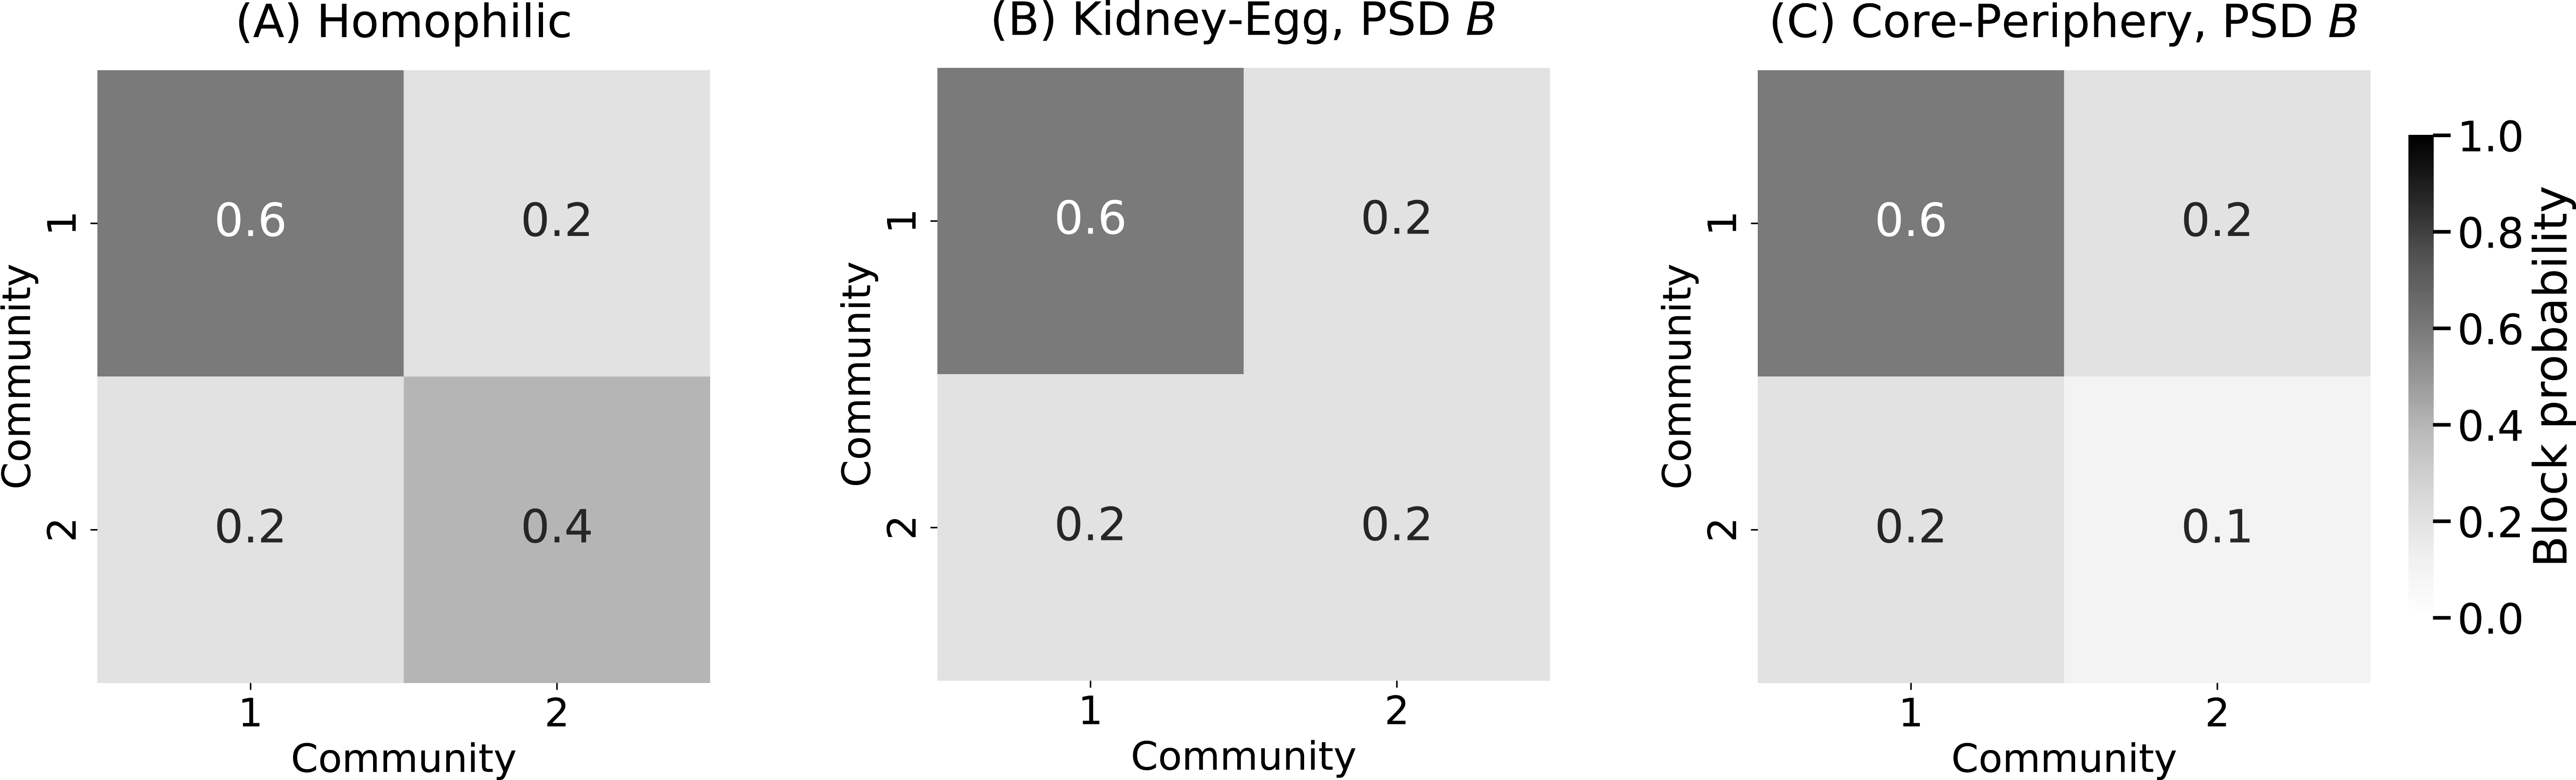
\includegraphics[width=\linewidth]{representations/ch5/Images/psd.png}
    \caption[PSD block matrices]{\textbf{(A)} a homophilic block matrix. \textbf{(B)} a positive semi-definite kidney-egg block matrix. \textbf{(C)} a positive semi-definite core-periphery block matrix.}
    \label{fig:ch5:psd_bmtx}
\end{figure}

\subsection{Planted partition block matrices}

A \textit{planted partition} block matrix is a block matrix where all of the on-diagonal entries are equal; that is, $b_{11} = b_{22} = \hdots = b_{KK}$ for all $K$ communities, and all of the off-diagonal entries are equal; that is, $b_{12} = \hdots b_{1K} = b_{21} = \hdots b_{2K} = \hdots b_{K1} = \hdots = b_{KK-1}$. In our case, this just means that $b_{11} = b_{22}$. 

Using the determinant condition and the fact that $b_{11} = b_{22}$, this implies that a planted partition is symmetric when $b_{11}^2 \geq b_{12}^2$. Since the entries of $B$ are probabilities and are hence non-negative, we can take square roots of both sides, and a sufficient condition is that $b_{11} \geq b_{12}$. When this criterion is satisfied, further clarify that the planted partition is a homophilic planted partition, because it fulfills the homophily criterion given in Section \ref{sec:ch5:psd_block:homophily}. 

We can generate an indefinite planted partition block matrix by just making an example where the block matrix has off-diagonal entries that exceed the on-diagonal entries, like this:


\begin{lstlisting}[style=python]
B_indef = np.array([[.1, .2], [.2, .1]])
block_mtx_psd(B_indef)
# False
\end{lstlisting}

\begin{figure}[h]
    \centering
    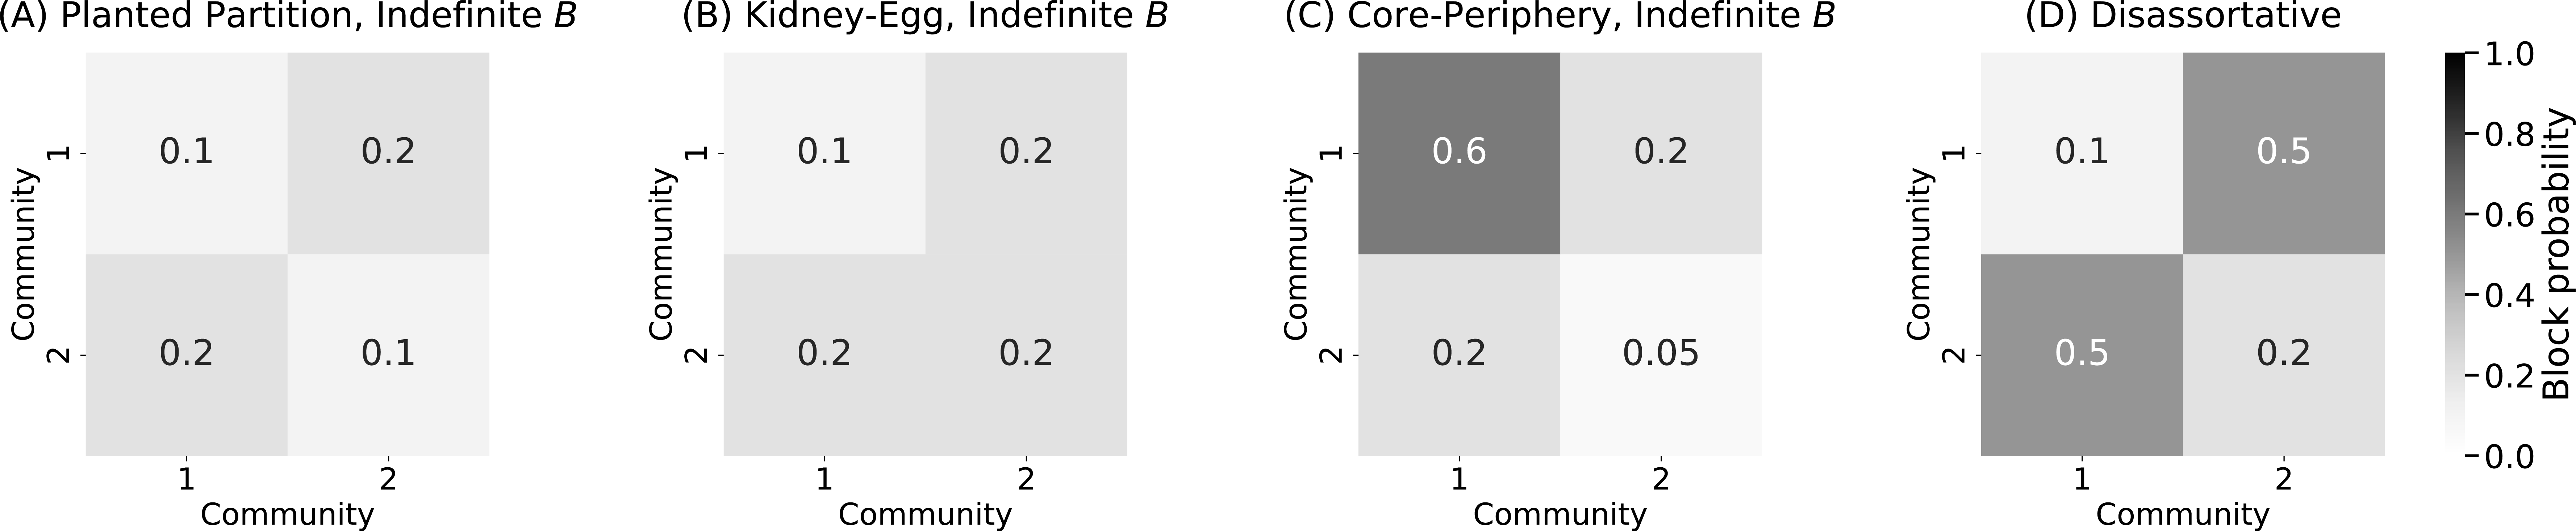
\includegraphics[width=\linewidth]{representations/ch5/Images/indef.png}
    \caption[Indefinite block matrices]{\textbf{(A)} an indefinite planted partition block matrix. \textbf{(B)} an indefinite kidney-egg block matrix. \textbf{(C)} an indefinite core-periphery block matrix. \textbf{(D)} a disassortative block matrix.}
    \label{fig:ch5:indef_bmtx}
\end{figure}

Which is shown in Figure \ref{fig:ch5:indef_bmtx}(A).

\subsection{Kidney-egg block matrices}

A \textit{kidney-egg} block matrix is a $2 \times 2$ block matrix where $b_{12} = b_{21} =  b_{22}$. For this matrix to be positive semi-definite, the determinant condition along with $b_{12} = b_{21} = b_{22}$ gives us that $b_{11}b_{12} \geq b_{12}^2$. Dividing through by $b_{12}$, we can see that the kidney-egg block matrices are positive semi-definite with the same conditions as planted partition block matrices; that is, $b_{11} \geq b_{12}$. Next, we generate two kidney-egg block matrices, one of which is indefinite and one of which is positive semi-definite. 

\begin{lstlisting}[style=python]
# a positive semi-definite kidney-egg block matrix
B_psd = np.array([[.6, .2], [.2, .2]])
block_mtx_psd(B_psd)
# True

# an indefinite kidney-egg block matrix
B_indef = np.array([[.1, .2], [.2, .2]])
block_mtx_psd(B_indef)
#False
\end{lstlisting}

We plot the positive semi-definite matrix in Figure \ref{fig:ch5:psd_bmtx}(B), and the indefinite matrix in Figure \ref{fig:ch5:indef_bmtx}(B).

\subsection{Core-periphery block matrices}

Core-periphery block matrices are block matrices where either $b_{11}$ or $b_{22}$ are greater than all of the other entries of the block matrix. This is called the core-periphery model because there are a group of nodes from a particular community (the \textit{core}) that tend to much more strongly connected than nodes that are not in that community (the \textit{periphery}). For instance, if community $1$ were the core community, $b_{11} > b_{22}$ and $b_{11} > b_{12}$, so the nodes of community $1$ tend to heavily associate with other core nodes. However, the nodes of community $2$ (the peripheral community) have far fewer connections both with other peripheral nodes and with core nodes. 

Core-periphery block matrices are a little bit harder to tie directly to positive semi-definiteness; the most precise that we can be is simply to say that $b_{11}b_{22} \geq b_{12}b_{21}$, which isn't particularly informative since that's literally the criterion for positive semi-definiteness that we gave.

Let's show how this condition works with some more examples:


\begin{lstlisting}[style=python]
# a positive semi-definite core-periphery block matrix
B_psd = np.array([[.6, .2], [.2, .1]])
block_mtx_psd(B_psd)
# True

# an indefinite core-periphery block matrix
B_indef = np.array([[.6, .2], [.2, .05]])
block_mtx_psd(B_indef)
# False
\end{lstlisting}

The positive semi-definite core-periphery block matrix is shown in Figure \ref{fig:ch5:psd_bmtx}(C), and the indefinite core-periphery block matrix is shown in Figure \ref{fig:ch5:indef_bmtx}(C).

\subsection{Disassortative block matrices}

A block matrix is \textit{disassortative} if $b_{12}$ and $b_{21}$ are greater than $b_{11}$ and $b_{22}$. By definition, disassortative block matrices are not positive semi-definite. This is because $b_{11}b_{22} < b_{12}b_{21}$, since all of the entries of $B$ are positive, and using the definition of the disassortative condition. Disassortative block matrices are a big conceptual ``thorn'' in the side of $RDPG_n(X)$ networks, as there is no possible way that we could use a disassortative block matrix to construct an equivalent $RDPG_n(X)$. 

To conceptualize what this would mean for a network, let's imagine that we have a simple network where the nodes are businesses, and each node is either a producer or a retailer. An edge exists in the network if a business relationship exists between two businesses. In general, producers will have business relationships with retailers, so the cross-community block probability $b_{12}$ is high. However, producers will not tend to have business relationships with their competitor producers, and retailers will not tend to have business relationships with their competitor retailers, so the within-community block probabilities $b_{11}$ and $b_{22}$ are comparatively low.

We can generate a disassortative block probability matrix like this:
\begin{lstlisting}[style=python]
# an indefinite disassortative block matrix
B = np.array([[.1, .5], [.5, .2]])
block_mtx_psd(B)
# False
\end{lstlisting}

A plot of an indefinite block matrix is shown in Figure \ref{fig:ch5:indef_bmtx}(D), and another example of a disassortative block matrix would be the indefinite planted partition block matrix shown in Figure \ref{fig:ch5:indef_bmtx}(B).

\subsection{How do we generate latent position matrices for $SBM_n(\vec z, B)$ random networks which are positive semi-definite?}
\label{sec:ch5:psd_block:lpm_fromsbm}
When a real matrix $W$ is positive semi-definite, as we mentioned, we can obtain a square-root matrix $\sqrt W$ where $W = \sqrt{W}\sqrt{W}^\top$. This matrix can be generated through a process known as the {Cholesky Decomposition} \cite{Horn2012Oct}. This process will come in handy over the next few sections when we are dealing with SBM block matrices and probability matrices that are positive semi-definite, and we want to obtain a latent position matrix. You can do this with \texttt{numpy}, like so:

\begin{lstlisting}[style=python]
# homophilic, and hence positive semi-definite, block matrix
B = np.array([[0.6, 0.2], [0.2, 0.4]])

# generate square root matrix
sqrtB = np.linalg.cholesky(B)

# verify that the process worked through by equality element-wise
# use allclose instead of array_equal because of extremely tiny
# numerical precision errors
np.allclose(sqrtB @ sqrtB.T, B)
# True
\end{lstlisting}

Next, we'll generate a community-assignment vector, and then use the code that we first produced in Section \ref{sec:ch5:ier:sbm_pmtx} to obtain a one-hot-encoding of the community-assignment vector. We can then use that to produce a latent position matrix, using the instructions from Equation \eqref{eq:ch5:ier:sbm_rdpg}, by taking $X = C\sqrt B$:

\begin{lstlisting}[style=python]
from graphbook_code import ohe_comm_vec

def lpm_from_sbm(z, B):
    """
    A function to produce a latent position matrix from a
    community assignment vector and a block matrix.
    """
    if not block_mtx_psd(B):
        raise ValueError("Latent position matrices require PSD block matrices!")
    # one-hot encode the community assignment vector
    C = ohe_comm_vec(z)
    # compute square root matrix
    sqrtB = np.linalg.cholesky(B)
    # X = C*sqrt(B)
    return C @ sqrtB

# make a community assignment vector for 25 nodes / community
nk = 25
z = [1 for i in range(0, nk)] + [2 for i in range(0, nk)]

# latent position matrix for an equivalent RDPG
X = lpm_from_sbm(z, B)
\end{lstlisting}

The resulting latent position matrix is shown along with the community assignment vector and the block matrix in Figure \ref{fig:ch5:psd_block:sbm_lpm}.

\begin{figure}[h]
    \centering
    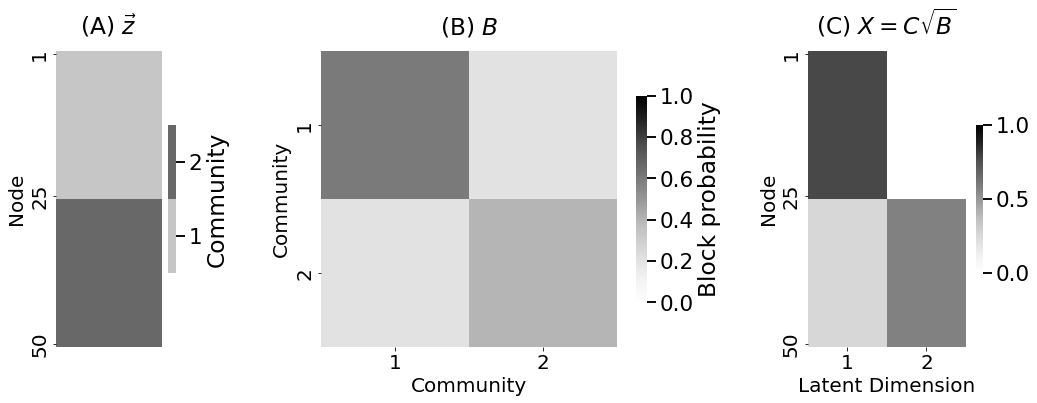
\includegraphics[width=\linewidth]{representations/ch5/Images/sbm_lpm.png}
    \caption[Latent position matrix for a positive semi-definite SBM]{\textbf{(A)} the community-assignment vector. \textbf{(B)} a homophilic block matrix, which is positive semi-definite. \textbf{(C)} the latent positions for an equivalent RDPG. Note that nodes with the same community have the same latent positions (rows of the latent position matrix $X$ in \textbf{(C)}).}
    \label{fig:ch5:psd_block:sbm_lpm}
\end{figure}

Finally, we can verify that the latent position matrix and the process described in Section \ref{sec:ch5:ier:sbm_pmtx} to generate the probability matrix for an SBM produce the same probability matrix:

\begin{lstlisting}[style=python]
from graphbook_code import generate_sbm_pmtx

# generate the probability matrices for an RDPG using X and SBM
P_rdpg = X @ X.T
P_sbm = generate_sbm_pmtx(z, B)

# verify equality element-wise
np.array_equal(P_rdpg, P_sbm)
# True
\end{lstlisting}

We can build a similar utility for the $DCSBM_n(\vec z, \vec \theta, B)$ random network, using Section \ref{sec:ch5:dcsbm:rdpg}, like so:

\begin{lstlisting}
def lpm_from_dcsbm(z, theta, B):
    """
    A function to produce a latent position matrix from a
    community assignment vector, a degree-correction vector,
    and a block matrix.
    """
    # X' = C*sqrt(B)
    Xp = lpm_from_sbm(z, B)
    # X = Theta*X' = Theta * C * sqrt(B)
    return np.diag(theta) @ Xp

# make a degree-correction vector
theta = np.tile(np.linspace(1, 0.5, 25), 2)
X_dcsbm = lpm_from_dcsbm(z, theta, B)
\end{lstlisting}

The resulting latent position matrix is shown along with the community assignment vector, the degree-correction vector, and the block matrix in Figure \ref{fig:ch5:psd_block:dcsbm_lpm}.

\begin{figure}[h]
    \centering
    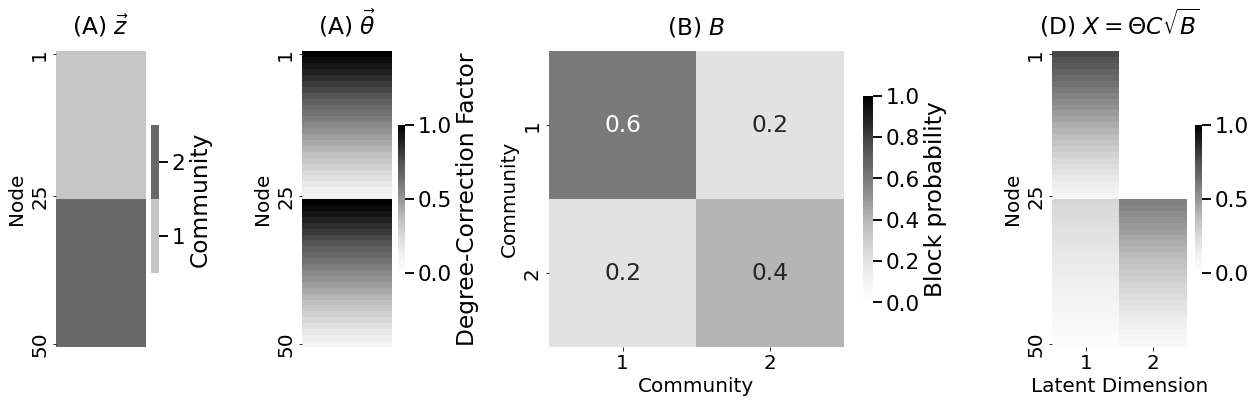
\includegraphics[width=\linewidth]{representations/ch5/Images/dcsbm_lpm.png}
    \caption[Latent position matrix for a positive semi-definite DCSBM]{\textbf{(A)} the community-assignment vector. \textbf{(B)} the degree-correction vector. \textbf{(C)} a homophilic block matrix, which is positive semi-definite. This block matrix is the same example shown in Figure \ref{fig:ch5:psd_bmtx}(A). \textbf{(D)} the latent positions for an equivalent RDPG. Note that nodes with the same community have similar latent positions, but appear to follow the same pattern in the degree-correction vector (large magnitudes for the first few nodes in each community, and smaller magnitudes for the last few nodes in each community).}
    \label{fig:ch5:psd_block:dcsbm_lpm}
\end{figure}

\subsection{Nodes in the same community (and with the same degree-correction factor) have the same latent position}
\label{sec:ch5:psd_block:same_lp}

As we learned in Equation \eqref{eq:ch5:ier:sbm_rdpg}, an $SBM_n(\vec z, \vec \theta, B)$ random network with a positive semi-definite block matrix (and hence a positive semi-definite probability matrix) can be represented as an $RDPG_n(X)$ random network, where the latent position matrix is:
\begin{align*}
    X = C \sqrt B
\end{align*}
For simplicity's sake, let's imagine that our SBM random network has two communities, and let's imagine the node $i$ is in community $1$. This means that the first row of the latent position matrix will be:
\begin{align*}
    \vec x_i^\top = \begin{bmatrix}
        1 & 0
    \end{bmatrix}\sqrt B.\numberthis \label{eqn:psd_block:c1}
\end{align*}
Now, let's imagine that we have another node, $i'$, which is also in community $1$. What is its latent position matrix?

That's right, you guessed it: it's the {exact same thing}, because the only thing that conveys information here is which community the node is in (which determines its row of the matrix $C$). What about a node $j$ in community $2$? This node will have a latent position of:
\begin{align*}
    \vec x_j^\top = \begin{bmatrix}
        0 & 1
    \end{bmatrix}\sqrt B. \numberthis \label{eqn:psd_block:c2}
\end{align*}
What would be the latent position vector for another node $j'$ also in community $2$? Again, it's the same thing. We could repeat this process for arbitrarily many communities; we just used the $2$-community case for simplicity. This example is shown in Figure \ref{fig:ch5:psd_block:sbm_lpm}(C). Notice that the rows of the latent position matrix (the latent positions for each node) are the same for nodes of the same community.

You can generalize this pattern to {any} nodes in the same community for an $SBM_n(\vec z, B)$ random network with a positive semi-definite block matrix: they will {always} have the same latent position vectors. 

We show an example of a homophilic block matrix matrix in Figure \ref{fig:ch5:psd_block:sbm_lpm}(A), which you learned above is positive semi-definite because it is homophilic. When we apply the conversion utility \texttt{lpm\_from\_sbm()}, we produce the latent position matrix in Figure \ref{fig:ch5:psd_block:sbm_lpm}(C). Notice that the rows for each of the two communities are equal. 

This insight provides us with the answer to the side note that we mentioned in Section \ref{sec:ch5:ier:rdpg_sbm}, that the street example provided a counter example indicating that not all $RDPG_n(X)$ random networks can be represented as $SBM_n(\vec z, B)$ random networks. For the street example, all of the latent positions are different for each node. If it were possible to represent the street example as an $SBM_n(\vec z, B)$ random network with $K < n$ communities, there would need to exist a group of nodes with the same latent position vector.

For a $DCSBM_n(\vec z, \vec \theta, B)$ random network, it's a little bit less clear what will happen. You learned in Section \ref{sec:ch5:dcsbm:rdpg} that the latent position matrix for a $DCSBM_n(\vec z, \vec \theta, B)$ when the block matrix (and hence also the probability matrix) was positive semi-definite was:
\begin{align*}
    X &= \Theta C \sqrt B.
\end{align*}
Intuitively, this feels very similar to the situation for the $SBM_n(\vec z, B)$ random network case, and it is.

Since $\Theta_i$ is diagonal, we can easily study what happens when you multiply $\Theta$ and $C$ together. It ends up working out like this:

\begin{align*}
    \Theta C &= \begin{bmatrix}
        \theta_1 c_{11} & \hdots & \theta_1 c_{1K} \\
        \vdots & \ddots & \vdots \\
        \theta_n c_{n1} & \hdots & \theta_n c_{nK}
    \end{bmatrix}
\end{align*}

All that you will end up doing is rescaling each row of $C$ (which was the one-hot encoding for each individual node's community assignment) by that node's degree-correction factor. Let's work back through the two community example as before, where $B$ is positive semi-definite (and hence, $\sqrt B$ exists). 

The latent position for a node $i$ in community $1$ is:
\begin{align*}
    \vec x_i^\top &= \begin{bmatrix}
        \theta_i & 0
    \end{bmatrix} \sqrt B,
\end{align*}
and for another node $i'$ also in community $1$ is:
\begin{align*}
    \vec x_{i'}^\top &= \begin{bmatrix}
        \theta_{i'} & 0 
    \end{bmatrix}\sqrt B.
\end{align*}

These two vectors are identical when $\theta_i = \theta_{i'}$. So, in some sense, the degree-correction factors $\theta_i$ or $\theta_{i'}$ are {rescaling} the latent position associated with community $1$ (which was given by Equation \ref{eqn:psd_block:c1}) for the node-specific latent position. 

Repeating this same process for two nodes $j$ and $j'$ in community $2$, we would get that:
\begin{align*}
    \vec x_j^\top &= \begin{bmatrix}
        0 & \theta_j
    \end{bmatrix} \sqrt B, \\
    \vec x_{j'}^\top &= \begin{bmatrix}
        0 & \theta_{j'} 
    \end{bmatrix}\sqrt B.
\end{align*}

Again, these two vectors are identical when $\theta_j = \theta_{j'}$. The degree-correction factors $\theta_i$ and $\theta_{j'}$ are {rescaling} the latent position associated with community $2$ (which was given by Equation \ref{eqn:psd_block:c2}) for the node-specific latent position. In this sense, we can conceptualize the degree-correction factor (with a positive semi-definite block matrix) as {rescaling} the latent position associated with a the community of that node. 

 This example is shown in Figure \ref{fig:ch5:psd_block:dcsbm_lpm}(D). Notice that the rows of the latent position matrix (the latent positions for each node) follow the same pattern (in magnitude) of the degree-correction vector in Figure \ref{fig:ch5:psd_block:dcsbm_lpm}(B). This is no accident: the degree-correction vector is  {rescaling} the latent position associated with the particular community.

 Even though the $DCSBM_n(\vec z, \theta, B)$ random networks are more complicated than the $SBM_n(\vec z, B)$ random networks due to the degree-correction factor, this still shows us that there are some $RDPG_n(X)$ random networks which cannot be represented as $DCSBM_n(\vec z, \theta, B)$ random networks with $K < n$. Working back to the street example again, there is no choice of degree-correction factors $\vec \theta$ which would allow us to rescale the latent position associated with a community and obtain the latent positions in the street example. Intuitively, you can conceptualize this result by noticing that the values of the latent dimensions from Figure \ref{fig:ch5:rdpg} for the street example have a pattern of taking opposites: as the value in latent dimension one increases, the value in latent dimension two decreases, and vice-versa(where all values of the latent position matrix were positive). Accounting for this with a degree-correction factor would require at a minimum that the pattern is the same; both would have to be simultaneously increasing or decreasing due to the fact that the latent position matrix has only positive entries.
 
So, we learned two things here:
\begin{enumerate}
    \item When the underlying random network is an $SBM_n(\vec z, B)$ and the block matrix is positive semi-definite, all nodes associated with the same community have the same latent position vector.
    \item When the underlying random network is an $DCSBM_n(\vec z, \vec \theta, B)$ and the block matrix is positive semi-definite, all nodes associated with the same community have the same latent position vector up to a rescaling by their degree-correction factor. If the nodes are in the same community and the degree-correction factor is the same, the nodes have the same latent position.
\end{enumerate}

\subsection{Some Thought Exercises}

This section should give you some good intuition on which block matrices are positive semi-definite in simple $2 \times 2$ cases. To solidify these concepts, we would strongly recommend that you go through the following exercises on your own:

\begin{enumerate}
    \item Choose a number of nodes $n$, and produce a community assignment vector to one of two communities for each of the $n$ nodes.
    \item Use the procedure that we outlined in Algorithm \ref{alg:ch5:sbm_pmtx} to generate a probability matrix for a given block matrix. Visualize the probability matrix, the adjacency matrix heatmap, and a layout plot of the networks alongside one another. 
    \item Generate a valid degree correction vector for the $n$ nodes. Use the procedure that we outlined in Algorithm \ref{alg:ch5:dcsbm_prob} to produce a probability matrix for the network, and generate a sample from the random network. Produce the same visualizations as above.
\end{enumerate}

\begin{floatingbox}[h]\caption{Core-periphery SBM and planted partition DCSBM equivalence}
Imagine that you have a $DCSBM_n(\vec z, \vec \theta, B)$, where the block matrix $B$ is a planted partition, and the degree-correction vector $\vec \theta$ has two unique values $u$ and $v$. These unique values are chosen such that whenever $z_i = 1$, $\theta_i = u$, and whenever $z_i = 2$, $\theta_i = v$. 
\begin{enumerate}
    \item Generate a visualization of the probability matrix.
    \item Use this visualization of the probability matrix to deduce that there exists a core-periphery block matrix $B'$ where $SBM_n(\vec z, B')$ and $DCSBM_n(\vec z, \vec \theta, B)$ have the same probability matrix.
    \item Find a function of $u$,$v$, and $B$ such that $B' = f(u, v, B)$. 
\end{enumerate}
Conclude that planted-partition DCSBMs with the degree-correction vector generated as-described are equivalent to core-periphery SBMs with a suitably chosen block matrix.
\end{floatingbox}
\newpage

\begin{floatingbox}[h]\caption{Degree-correction factor ``stretch'' latent positions}
\label{box:ch5:psd_block:stretch}
Take a positive semi-definite block matrix $B$ associated with a $2$-community $SBM_n(\vec z, B)$ random network (for instance, the homophilic block matrix we used in the examples here). Take a range of values for $\theta$, from $0$ to $1$ in $0.1$ increments, and compute the latent position matrix for the $SBM_n(\vec z, B)$ random network. This will give you a $n \times 2$-dimensional latent position matrix.
\begin{enumerate}
    \item Take the latent position associated with community $1$ (it will be the same for all nodes in community $1$, and will be a $2$-dimensional point $\vec x$). Rescale it for all values of $\theta$. 
    \item Next, plot $\theta \vec x$, for all values of $\theta$. 
    \item Conclude that $\theta$ is ``stretching'' $\vec x$ along a straight line.
    \item Repeat for the latent position $\vec y$ associated with community $2$.
\end{enumerate}
Conclude that degree-correction factors for $DCSBM_n(\vec z, \vec \theta, B)$ random networks``stretch'' the latent positions of $SBM_n(\vec z, B)$ random networks along a straight line, depending on the value of $\theta$. 
\end{floatingbox}